\begin{figure}[H]
    \centering
    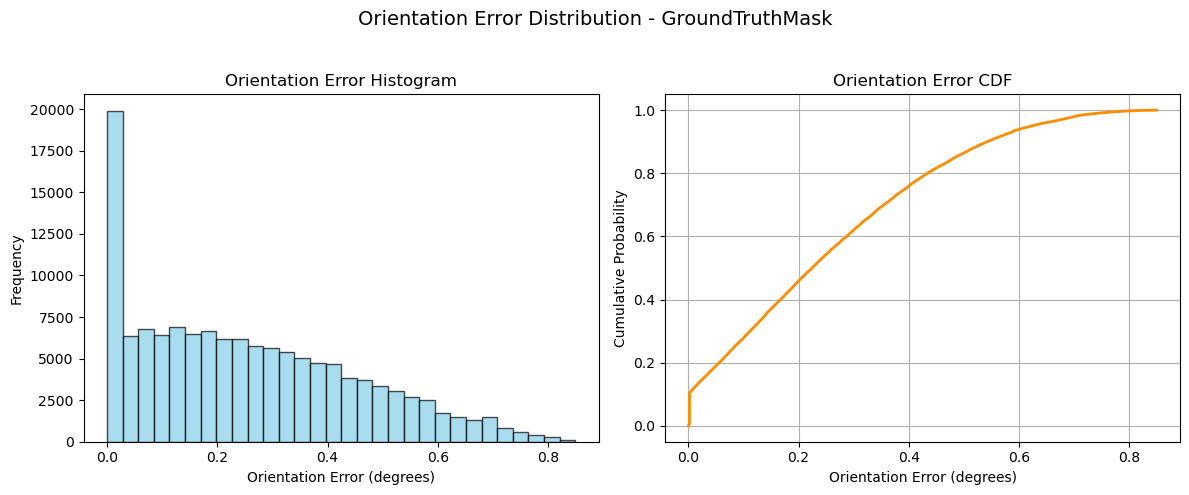
\includegraphics[width=\textwidth]{figures/appendix/gt_orientation_error_distribution.png}
    \caption{
        Baseline orientation error between ground-truth (GT) angles from the CSV annotations and those computed from the GT segmentation masks.
        (\textbf{Left}) Histogram of the error in degrees.
        (\textbf{Right}) Cumulative distribution function (CDF) of the error.
        The error originates from discretizing continuous ellipses into pixel masks and represents the minimal possible error achievable.
    }
    \label{fig:gt-baseline-error}
\end{figure}

\begin{figure}[H]
    \centering
    \includegraphics[width=0.49\textwidth]{figures/appendix/Unet3 Signed Orientation Error Distribution.png}
    \hfill
    \includegraphics[width=0.49\textwidth]{figures/appendix/Unet3 Orientation Error vs GT-Angle.png}
    \caption{
        Analysis of orientation errors for UNet3.
        (\textbf{Left}) Distribution of signed orientation errors showing no substantial bias, with errors approximately symmetrical around zero.
        (\textbf{Right}) A hexbin plot showing the distribution of absolute orientation error versus the ground-truth angle.
        Errors appear to be uniformly distributed across the range of ground truth angles.
        The concentration of points at \qty{0}{\degree} reflects the overrepresentation of \qty{0}{\degree} GT angles in the dataset, but the error pattern remains similar at other angles.
    }
    \label{fig:appendix_unet3_orientation}
\end{figure}

\begin{figure}[H]
    \centering
    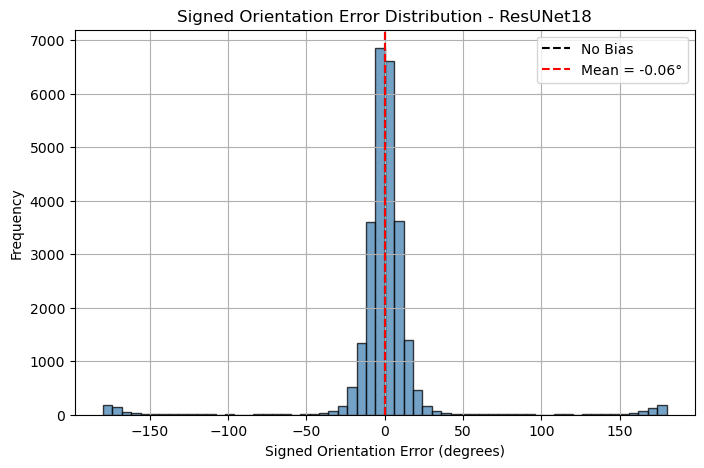
\includegraphics[width=0.49\textwidth]{figures/appendix/ResUNet18 Signed Orientation Error Distribution.png}
    \hfill
    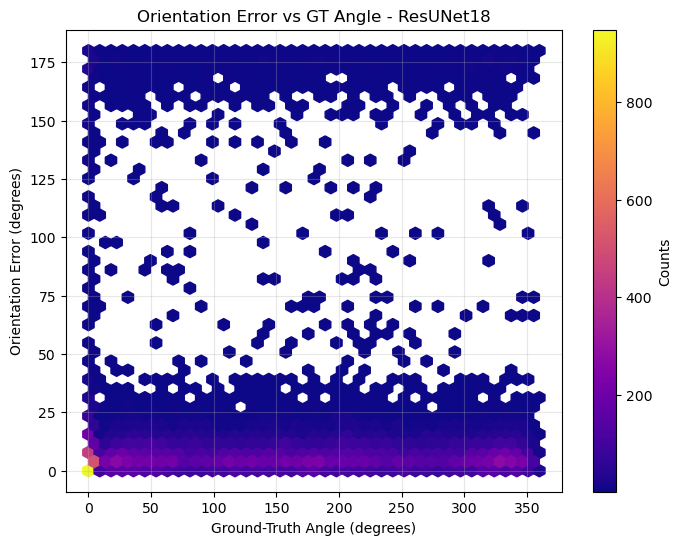
\includegraphics[width=0.49\textwidth]{figures/appendix/ResUNet18 Orientation Error vs GT-Angle.png}
    \caption{
        Analysis of orientation errors for ResUNet18.
        (\textbf{Left}) Distribution of signed orientation errors, again showing no systematic bias and symmetric distribution around zero.
        (\textbf{Right}) Hexbin plot of absolute orientation error versus ground‑truth angle, indicating no particular GT angle is associated with higher or lower errors.
        The dense region at \qty{0}{\degree} reflects dataset imbalance rather than a modeling issue.
    }
    \label{fig:appendix_resunet18_orientation}
\end{figure}

\begin{figure}[htbp]
    \centering
    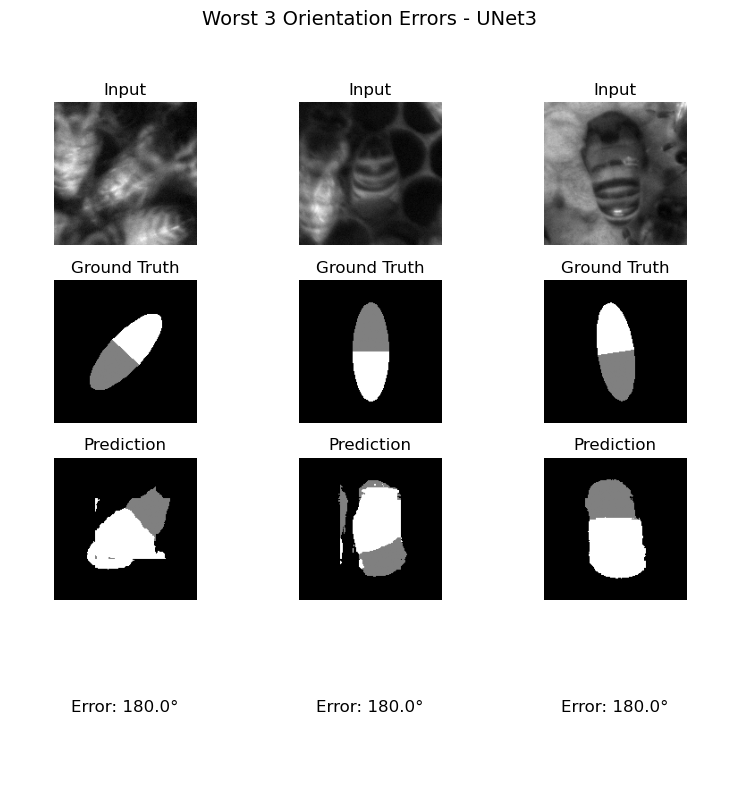
\includegraphics[width=0.49\textwidth]{figures/results/5 - fails/UNet3 Worst Orientation Errors.png}
    \hfill
    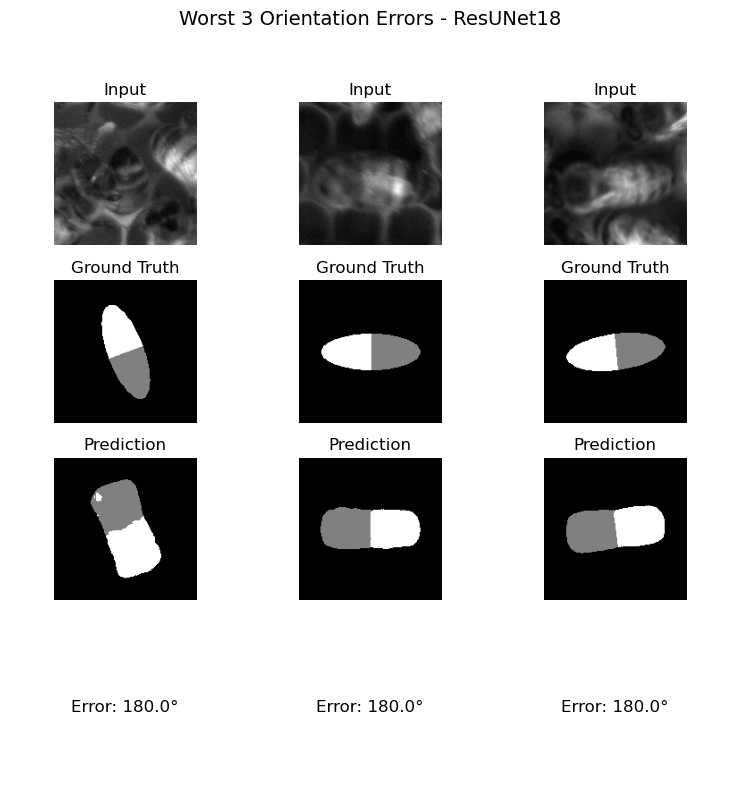
\includegraphics[width=0.49\textwidth]{figures/results/5 - fails/ResUNet18 Worst Orientation Errors.png}

    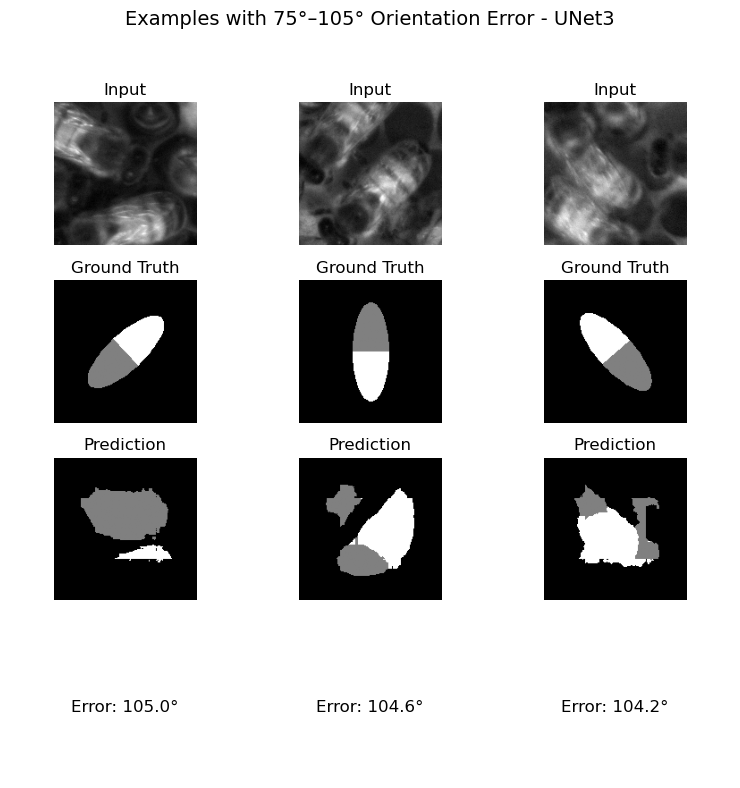
\includegraphics[width=0.49\textwidth]{figures/results/5 - fails/UNet3 Orientation Errors 90deg Range.png}
    \hfill
    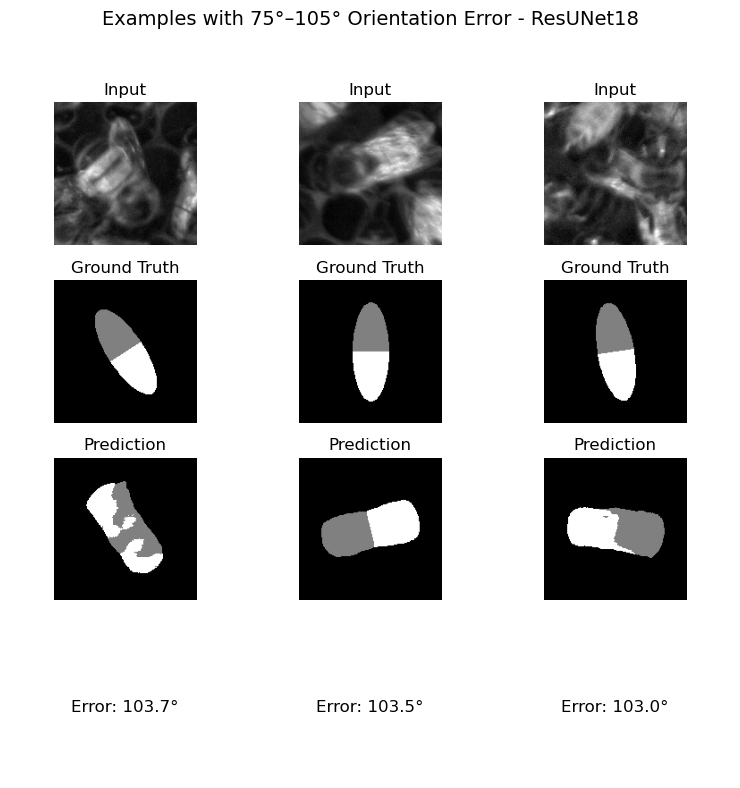
\includegraphics[width=0.49\textwidth]{figures/results/5 - fails/ResUNet18 Orientation Errors 90deg Range.png}
    \caption{
        Qualitative failure cases for UNet3 (\textbf{left}) and ResUNet18 (\textbf{right}), with the worst absolute orientation errors (\textbf{top row}) and examples with errors around \qty{90}{\degree} (\textbf{bottom row}).
        Each panel shows the input image, ground‑truth mask, predicted mask, and measured error.
        In the worst (\qty{180}{\degree}) cases, annotations are often flipped, while model predictions remain plausible.
        Around \qty{90}{\degree}, both models struggle in highly cluttered or ambiguous scenes, but ResUNet18 still produces more coherent segmentations than UNet3.
    }
    \label{fig:failure_modes}
\end{figure}